%%%%%latex preamble%%%%%
\documentclass[titlepage]{article}\usepackage[]{graphicx}\usepackage[]{color}
%% maxwidth is the original width if it is less than linewidth
%% otherwise use linewidth (to make sure the graphics do not exceed the margin)
\makeatletter
\def\maxwidth{ %
  \ifdim\Gin@nat@width>\linewidth
  \linewidth
  \else
  \Gin@nat@width
  \fi
}
\makeatother

\usepackage{rotating}
\usepackage{listings}
\definecolor{mygreen}{rgb}{0,0.6,0}
\definecolor{mygray}{rgb}{0.5,0.5,0.5}
\definecolor{mymauve}{rgb}{0.58,0,0.82}
\lstset{ %
  backgroundcolor=\color{white},   % choose the background color; you must add \usepackage{color} or \usepackage{xcolor}
  basicstyle=\footnotesize,        % the size of the fonts that are used for the code
  breakatwhitespace=false,         % sets if automatic breaks should only happen at whitespace
  breaklines=true,                 % sets automatic line breaking
  captionpos=b,                    % sets the caption-position to bottom
  commentstyle=\color{mygreen},    % comment style
  deletekeywords={...},            % if you want to delete keywords from the given language
  escapeinside={\%*}{*)},          % if you want to add LaTeX within your code
  extendedchars=true,              % lets you use non-ASCII characters; for 8-bits encodings only, does not work with UTF-8
  frame=single,                    % adds a frame around the code
  keepspaces=true,                 % keeps spaces in text, useful for keeping indentation of code (possibly needs columns=flexible)
  keywordstyle=\color{blue},       % keyword style
  language=Python,                 % the language of the code
  morekeywords={*,...},            % if you want to add more keywords to the set
  numbers=left,                    % where to put the line-numbers; possible values are (none, left, right)
  numbersep=5pt,                   % how far the line-numbers are from the code
  numberstyle=\tiny\color{mygray}, % the style that is used for the line-numbers
  rulecolor=\color{black},         % if not set, the frame-color may be changed on line-breaks within not-black text (e.g. comments (green here))
  showspaces=false,                % show spaces everywhere adding particular underscores; it overrides 'showstringspaces'
  showstringspaces=false,          % underline spaces within strings only
  showtabs=false,                  % show tabs within strings adding particular underscores
  stepnumber=2,                    % the step between two line-numbers. If it's 1, each line will be numbered
  stringstyle=\color{mymauve},     % string literal style
  tabsize=2,                       % sets default tabsize to 2 spaces
  title=\lstname                   % show the filename of files included with \lstinputlisting; also try caption instead of title
}
\usepackage{alltt}
\usepackage[sc]{mathpazo}
\usepackage{amsmath, amsthm, amssymb}
\usepackage{graphicx}
\usepackage[T1]{fontenc}
\usepackage{geometry}
\geometry{verbose,tmargin=2.5cm,bmargin=2.5cm,lmargin=1.5cm,rmargin=1.5cm}
\setcounter{secnumdepth}{2}
\setcounter{tocdepth}{2}
\usepackage{float}
\usepackage{bm}
\usepackage{tikz}
\usetikzlibrary{arrows,automata}

 %changes default sectioning commands -> 1,a, etc.
%\usepackage{breakurl}
\renewcommand{\thesubsection}{(\alph{subsection})}
\renewcommand{\thesubsubsection}{\roman{subsection}.}

\usepackage{url}
\usepackage{hyperref}
\hypersetup{pdfborder = {0 0 0}}

%%% Header and Footer %%% 
\usepackage{lastpage}
\usepackage{fancyhdr}
%%% fancy pages for all non-title and chapter heading pages
\pagestyle{fancy}
%%% puts a line in the footer
\renewcommand{\footrulewidth}{0.4pt}
%%% adds a reference to the last page to give a running page count
\fancyfoot[R]{\thepage of \pageref{LastPage}} %requires lastpage
%%%% adds author name to bottom left
\fancyfoot[L]{\textit{Gonzales, Darki, Navada; Group 16}}
%%% empty center footer
\fancyfoot[C]{}

%%% Adds class name to left header
\fancyhead[L]{\textit{Theory of Computation}}
%%% Adds document name to right header
\fancyhead[R]{\textit{Homework 2: More fun with automata}}

\IfFileExists{upquote.sty}{\usepackage{upquote}}{}

\begin{document}

\title{More Fun With Automata \\ Homework 2, CS500, Fall 2014}
\author{Aaron Gonzales, Ahmad Darki, Manasa Navada \\ group 16}
\maketitle


%%%%%%%%%%%%%%%%%%%%%%%%%%%%%%%%%%%%%%%%%%%%%%%%
\section*{Ex 7}
\begin{quote}
  \textbf{Show that if $L$ is regular then $L^*$ is regular. Why does it not suffice
  to use the fact that the regular languages are closed under concatenation and
  union?}
\end{quote}
\subsubsection*{Answer:}
We know that $L* = \epsilon \cup L \cup LL \cup \dots$, the enumerated set of
all possible combinations of strings made up of the language $L$. We also know
that for a language to be regular, there must be some DFA or NFA that can
accept it. 

If we let $M_L$ be the machine that recognizes langague $L$, then let $M_{L^*}$
be the machine that recognizes $L^*$. To construct $M_{L^*}$, add a new start
state $S'$ that is also an accepting state to $M_L$. Connect $S'$ to $M_L$ with
an $\epsilon$ transition and add another $\epsilon$ edge out of $M_L$ such that
it connects to $S'$. This machine can accept any possible combinatins of valid
instances of $L$ and includes $\epsilon$, showing that $L^*$ is indeed regular. 

Since we are adding an $\epsilon$ transition, concatenation and union do not
cover $\epsilon$ closure and we need to account for that.


%%%%%%%%%%%%%%%%%%%%%%%%%%%%%%%%%%%%%%%%%%%%%%%%

\section*{Ex 8}
\begin{quote}
  \textbf{Given a string $w$ , let $w^R$ denote $w$ written in reverse.
    Given a language $L$, let $L^R = \{w^R | w \in L \}$. Prove that $L$ is regular if and
    only if $L^R$ is regular. Why is this harder to prove with DFAs?}
\end{quote}
\subsubsection{Answer:}
We know that a language is regular if there is a DFA that can accept it. This
tells us that in order to prove $W^R$'s regularity, there must be some DFA that
can accept it. Generally put, we can map our current DFA to a DFA that can
accept the new reversed language by modifying the start state, accepting
states, and transition functions as follows, which will be formalized below.

\begin{proof} 
	Let $M = \{S, A, s^0, S^{yes}, \delta\}$ be the machine that recognizes $L$.
	Let $M' = {S',A',S^{0'}, S^{yes'}, \delta*'}$ be the NFA that recognizes
	$L^R$, constructed as below:

	Let $S_{new} \in S$ be a new start state and connect it to all $s \in S^{yes}$
	with an $\epsilon$ label. 
	Make $S^0$ into an $S^{yes'}$. 
	Make $s \in S^{yes} \to S'$ (make accepting states into normal states).
	Make $S^{0} \to S^{yes'}$ (make the original intial state into the sole
	accepting state.

	This new NFA will only accept langagues that begin in the first char of the
	$w^R$ and end in the last char of $w^r$. As we have constructed an NFA that
	recognizes this $L^R$, we can deduce that that $L^R$ is regular, meaning
	that $L \Leftrightarrow L^R$.
\end{proof}

The NFA epsilon ability allows us to more easily create new NFAs from
exisisting automata.


%%%%%%%%%%%%%%%%%%%%%%%%%%%%%%%%%%%%%%%%%%%%%%%%

\section*{Ex 9}
\begin{quote}
  \textbf{A for-all NFA is one such that $L(M)$ is the set of strings where every
  computation path ends in an accepting state. Show how to simulate an for-all
  NFA with a DFA, and thus prove that a language is recognized by some for-all
  NFA if and only if it is regular.}
\end{quote}

\subsubsection*{Answer:}
This is similar to converting any NFA to a DFA. 
let \[ A_n = \{ Q, q_0 \in Q, F \subseteq Q, \delta : Q \times \Sigma \to P(Q) \} \]
  be the $\forall$ NFA we wish to convert.

Let \[ A_d = \{Q' = \mathcal{P}(Q), \{ q_0 \}, \delta'(S,a) = \cup_{q \in S}
\delta(q,a), F' = \{ S \subseteq Q : S \cap F \neq \varnothing \} \} \]
be the DFA to which we are mapping $A_n$.

note that
\begin{align*}
  Q' =& \mathcal{P}(Q)& Q' \text{ is power set of } Q \\ 
  F' =& \{ S \subseteq Q : S \cap F \neq \varnothing \} \} &\text{ DFA accepting states
  as subsets of Q with all elements accepting } 
\end{align*}
So all of the DFA's accepting states are on a computation path and that the
All-paths NFA recognizes a regular language as we have build its DFA.



%%%%%%%%%%%%%%%%%%%%%%%%%%%%%%%%%%%%%%%%%%%%%%%%

\section*{Ex 10}
\begin{quote}
  \textbf{ A parity finite-state automaton, or $PFA$ for short, is like an
    $NFA$ except that it accepts a string $w$ if and only if the number of
    accepting paths induced by reading $w$ is odd. Show how to simulate a $PFA$
    with a $DFA$, and thus prove that a language is recognized by a $PFA$ if
    and only if it is regular. Hint: this is a little trickier than our
  previous simulations, but the number of states of the $DFA$ is the same.}
\end{quote}

\subsubsection*{Answer:}
Assume an $NFA$ being regular:

\[ 
  M_2 = (S_2, A, S^0_2, S^{yes}_2, \delta_2)
\]
From this $NFA$ we will have a $DFA$ as:

\[ 
  M = (S, A, S^0, S^{yes}, \delta)
\]

Where $S = 2^{S_2}$, $S^{yes} = {S^{yes}_2}$, $\delta(T, a) = \cup_{t\in T}
\delta_2(t, a)$, and $S^{yes} = \{T\cap S^{yes}_2\}$ in which this $DFA$ is
regular as well. For this problem we need to prove that for an odd number of
$\delta_2(S^0_2, w) = s^{yes}_2 \in S^{yes}_2$ we will be able to make another
$DFA$. From this we know that there will be an odd number of transitions of
$\delta_2(S^0_2, w)$ which means $|w|$ is an odd number as in
$w=w_1w_2...w_(2n+1)$.  







\section*{Ex 11} 
\begin{quote} \textbf{Given finite words $u$ and $v$, say that
    a word $w$ is an interweave of $u$ and $v$ if I can get $w$ by peeling off
    symbols of $u$ and $v$, taking the next symbol of $u$ or the next symbol of
    $v$ at each step, until both are empty. (Note that w must have length $|w|
    = |u| + |v|$.) For instance, if $u = cat$ and $v = tapir$, then one
    interleave of $u$ and $v$ is $w = ctaapitr$. Note that, in this case, we
    don't know which $a$ in $w$ came from $u$ and which came from $v$. Now
    given two languages $L_{1}$ and $L_{2}$, let $L_{1} \wr L_{2}$ be the set
    of all interweaves $w$ of $u$ and $v$, for all $u \in L_{1}$ and $v \in
    L_{2}$. Prove that if $L_{1}$ and $L_{2}$ are regular, then so is $L_{1}
    \wr L_{2}$.}
\end{quote}
\subsubsection*{Answer:}

The machine for $L_1$ can be defined as:

\[ 
	M_{1} = \{S_{1}, A, S_{1}^0, S_{1}^{yes}, \delta_{1} \}
\]

and the machine for $L_2$ as:

\[ 
	M_{2} = \{ S_{2}, A, S_{2}^0, S_{2}^{yes}, \delta_{2} \}
\]

The product construction of the two languages allows us to run them in
parallel. Let $L' = L_1 \times L_2$ to be the \textit{Cartesian product} of the
two languages $L_1$ to $L_2$, with its machine defined as:

\[ 
	M' = \{ S' = \{ S_{1} \times S_{2} \} , A, S'^0 = \{ S_{1}^0 \cup  S_{2}^0
\}, S'^{yes} = \{ S_{1}^{yes} \cup S_{2}^{yes} \} , \delta' = \{ \delta_{1}
\times \delta_{2} \} \}
\]


Now, in order to handle the potential for various combinations of valid
interweaves, we need to use the power set of $L'$, which would result in this
final machine, $M$, that  recognizes $L_1 \wr L_2$.

\begin{align*}
	M =& (S, A, S_0, S^{yes}, \delta) \\
	S =& \mathcal{P}(S')  \\
	S_0 =& S_{L_1}^0 \cup S_{L_2}^0 \\
	S^{yes} =& s \in S'^{yes} \\ 
	\delta =& \{ \{\delta_1, S_n, a \in A \}, \{ \delta_2, S_n, a \in A \} \} 
\end{align*}

This allows us to accept words that are valid in and order of $M_1$  and $M_2$,
such as the word ``cat'' $\in L_1$ and ``cat'' $\in L_2$ allows us to accept
the first word in any valid accpeting state of $M_1$ and continue weaving it
with the rest of the possible states of $M_2$, e.g., ``cacatt''. 

%%%%%%%%%%%%%%%%%%%%%%%%%%%%%%% 

%%%%%%%%%%%%%%%%%%%%%%%%%%%%%%% EX 12 %%%%%%%%%%%%%%%%%%%%%%%%%%%%%%%%%%%%
\section*{Ex 12}
\begin{quote}
	\textbf{Given a language $L$, let $L_{1/2}$ denote the set of words that can appear
    as first halves of words in $L$:}
    \[ L_{1/2} = \{ x | \exists y : |x| = |y| \text{ and } x y \in L \} \]
    
  \textbf{where $|w |$ denotes the length of a word $w$ . Prove that if $L$ is
      regular, then $L_{1/2}$ is regular. Generalize this to $L_{1/3}$, the set of
      words that can appear as middle thirds of words in $L$:}
  \[ L_{1/3} = \{ y | \exists x,z : |x| = |y| = |z|\,  \text{and } x y z \in L \} \]
  
\end{quote}
\subsubsection*{Answer A:}
We know that $|x| = |y|$ and must show that the set of words in $L_{1/2}$ can
be represented by a DFA to be proved regular. FA's limit us in that we cannot
go back in time or record with external memory, and we may not know how large a
word $w$ is before it is read. As such, we must (A) build a FA that allows us to
give $|x| = |y|$ and allows us to verify that (B) $xy \in L$. This is complicated
but not impossible.

Chris Moore's hint about River Song and the Doctor is a reference to Dr. Who,
in which the characters are moving toward each other in time, one going
forward and the other going backward. Given that hint, let us construct a FA
that allows us to accomplish A and B, mostly given by the product construction
of two FAs.

\begin{proof}
	Let us define two FAs:
        \footnote{teammates, My notation here may be slightly wonky (the
          NFA/DFA notation needs cleaning and I will gladly
        put in a figure to help explain this in better detail regarding the overlap of
        the boundary states for the words on both parts a and b}
	\begin{align}
		M =& \{Q, \Sigma, \delta, S_0, S^{yes}\} \\
		M^R =& \{ Q^R, \Sigma, \delta^R, S^{yes^R} \} \\
		Q^R = & Q \cup \{S_{0}^R \}
	\end{align}
	$M$ is the DFA which recognizes $L$ and $M^R$ is the NFA that recognizes
	$L^R$. We have seen that the reverse operator is closed under
	regularity. $Q^R$ is the union of states of $M$ and acepting states of
	$L^R$.
        Now introduce $M_{1/2}$, the machine that recognizes $L_{1/2}$, which
        is the product of $M \times M^R$ and we define all of $M_{1/2}$
        member's below.
        
        \begin{align}
          M_{1/2} = & M \times M^R \\ = &  \{ Q_{1/2}, \Sigma, \delta_{1/2}, S_{o_{1/2}}, S_{1/2}^{yes}  \} & \\
          Q_{1/2} = & Q \times Q^R \hfill & \text{States} \\ 
          \delta_{1/2} = & \{ (q_1, q_2), a\} = \cup_{c \in \Sigma} \{ \delta (q_1, a), \delta^R (q_2, c)\} &\text{ transition function }\\ 
          S_{0_{1/2}} = & \{ S_0, S_0^R \} & \text{ initial states} \\
          S^{yes}_{1/2} = & \{ (q1,q) | q \in Q \} & \text{ accepting states}
	\end{align}

        Our new machine, $M_{1/2}$ will read the string $w \in L$ and only
        accept it if the strings $x,y$ are equal in length and are a part of
        this new $L_{1/2}$ language. 
\end{proof}

\subsection{Answer B}
Proving this for $L_{1/3}$ would involve repeating the process from above and
getting a triple product construction for the three FA for which we have
interest, though the construction of this is laborious. 
A possible proof by induction for an $L_{1/n}$ for which any word in the
language can be chopped into $n$ discreet and equal chunks could follow. 

\begin{proof}
  Via induction over the size of a word 
  \[ |x_1|, |x_2|, \dots |x_n| | \sum_{i=1}^n |x_i| = w \in L \]
  , where $L$ is regular and $|w|\%n=0 $ .

\end{proof}



%%%%%%%%%%%%%%%%%%%%%%%%%%%%%%%%%%%%%%%%%%%%%%%%

\section*{Ex 13}
\begin{quote}
  \textbf{Show that if $u \sim_L v$ , then $u a \sim_L v a$ for any $a \in A$.}
\end{quote}
\subsubsection{Answer:}

\begin{proof}
L-equivalence is defined by Definition 3 \footnote{Automata notes} as given some
language $L \subseteq A^*$, $u,v \in A^*$ are $u \sim_L v$ if $\forall w \in
A^*\, \, uw \in L \text{ iff } vw \in L$. 
Since this is a forall notion, we can say that this would include words $w = ax$
or a word comprised with a prefix a on x. $\forall x, uax \in L \text{ iff } vax \in
L \implies ua \sim_L va$.
\end{proof}


%%%%%%%%%%%%%%%%%%%%%%%%%%%%%%%%%%%%%%%%%%%%%%%%
\section*{Ex 14}
\begin{quote}
  \textbf{Describe the equivalence classes of the three languages from Exercise
  2. Use them to give the minimal DFA for each language, or prove that the DFA
  you designed before is minimal.}
\end{quote}
t
\subsection*{Part 1}
\subsubsection{Answer:}
\begin{figure}[htp]
	\centering
	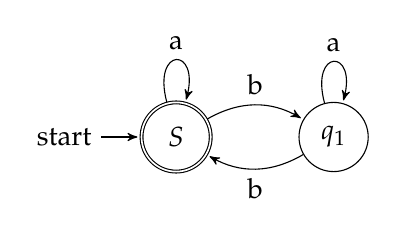
\begin{tikzpicture}[>=stealth',shorten >=1pt,auto,node distance=2cm]
		\node[initial,state, accepting] (S)  {$S$};
		\node[state] (q1) [right of=S]  {$q_1$};


		\path[->] (S)  edge [loop above] node {a} (S)
		edge [bend left] node {b} (q1)
		(q1) edge [bend left]  node {b} (S)
		edge [loop above] node {a} (q1);
	\end{tikzpicture}
	\caption{DFA for Exercise $2(a)$, the set of words in $\{a,b\}* $ with an
			even number of b's.}
  \end{figure}

  We know that there are only two equivalence classes, thanks to this DFA being
  in its minimal state. 

  \[ \{ z | \forall w \in L \Leftrightarrow zw \in L \} \]
  Note that the above describes the class with $z$ having even b's and $w$
  having even b's. 

  we have a class $\{bb\}$, the class where we have an even number of b's and a
  class $\{b\}$ in which we have an odd number of b's. All other combinations
  in the language do not matter.


  \subsection*{Part 2}
\begin{quote}
  \textbf{Describe the equivalence classes of the three languages from Exercise
  2. Use them to give the minimal DFA for each language, or prove that the DFA
  you designed before is minimal.}
\end{quote}
\subsubsection{Exercise 2.2: The set of strings in $\{a, b, c\}^*$ where there is no $c$ anywhere to the left of an $a$.}
As it has been proven that the following DFA is a minimal, with respect to the number of states the \textit{equivalence class} are 3 as followed:

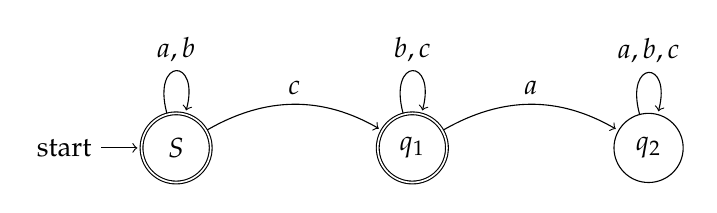
\begin{tikzpicture}[shorten >=1pt,auto,node distance=3 cm, scale = 1, transform shape]


\node[initial,state,accepting] (S)                                    {$S$};
\node[state,accepting]         (B) [right of=S]                       {$q_1$};
\node[state]                   (C) [right of=B]					      {$q_2$};

\path[->]
      (S) edge [loop above] node [align=center]  {$ a, b $} (S)
      (S) edge [bend left]       node {$ c $} (B)
      (B) edge [loop above] node [align=center]  {$ b, c $} (B)
      (B) edge [bend left] node [align=center]  {$ a $} (C)
      (C) edge [loop above] node [align=center]  {$ a, b, c $} (C);
\end{tikzpicture}

\begin{enumerate}
  \item $[\epsilon] = [a] = [ab] = [aba]$, The set of strings in $w$ without any $c$.
  \item $[c] = [cb] = [cbc]$, The set of strings in $w$ starting with $c$.
  \item $[c] = [cb] = [cbc] = [cbcb] = [cbcba]$, The set of strings in $w$ where there is $c$ to the left of $a$
\end{enumerate}




  \subsection*{Part 3}
  \begin{quote}
	  \textbf{ The set of strings in $\{0,1\}^*$ that encode, in binary,
  an integer w that is a multiple of 3. Interpret the empty string $\epsilon$
  as the number zero. }
  \end{quote}
  \subsubsection{Answer:}
  A minimal DFA for this language has three states. Each state represents the
  reminder of the number when it is divided by 3.
  The equivalence classes for this language are:  
  \begin{enumerate}
	\item  w containing the reminder 0. (Also the start state and accepting state)
	\item  w containing the reminder 1.
	\item  w containing the reminder 2.
\end{enumerate}
  Considering the following transition between these gives the following DFA.

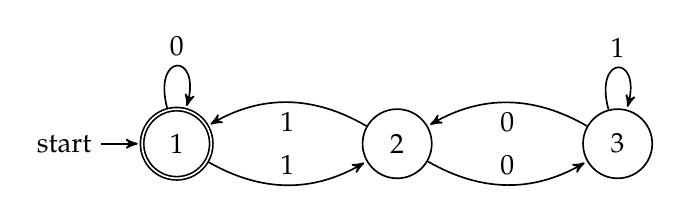
\begin{tikzpicture}[->,>=stealth',shorten >=1pt,auto,node distance=2.8cm,
                    semithick]

  \node[initial,state, accepting] (A) {$1$};
  \node[state]         (B) [right of=A] {$2$};
  \node[state]         (C) [right of=B] {$3$};

  \path (A) edge [bend right] node {1} (B)
            edge [loop above] node {0} (A)
        (B) edge [bend right] node {1} (A)
            edge [bend right] node {0} (C)
        (C) edge [bend right] node {0} (B)
            edge [loop above] node {1} (C);
\end{tikzpicture}

Hence it is proved that the DFA we designed in HW1 is minimal. 


%%%%%%%%%%%%%%%%%%%%%%%%%%%%%%%%%%%%%%%%%%%%%%%%
\section*{Ex 20}
\begin{quote}
  \textbf{Consider the language}
  \[ L_{a=b,c=d } = \{ w \in \{a,b, c ,d \}^* \, | \#_a (w) = \#_b (w) \text{ and }
    \#_c (w) = \#_d (w )
  \]
  
\textbf{What are its equivalence classes? What does its minimal infinite-state machine
look like?}
\end{quote}

\subsubsection{Answer:}
Clearly, we can see that we would require an infinite number of states to
count the number of each letter in $A$. Formally, we can see the equivalence
classes of $L_{a=b,c=d}$ as such:

Consider the set of words

\[ \{ a^i | i \geq 0 \} = \{ \epsilon, a, aa, aaa, \dots\} \]. 
If $i \neq j \implies a^i \not \sim a^j$, as 
\[ a^ib^i \in L_{a=b} \text{, but } a^jb^i \notin L_{a=b} \]

We need a similar set of words for c:
\[ \{ c^n | n \geq 0 \} = \{ \epsilon, c, cc, ccc, \dots\} \]. 
If $i \neq j \implies c^i \not \sim c^j$, as 
\[ c^nd^n \in L_{c=d} \text{, but } c^md^n \notin L_{c=d} \]

Each possible $i,n$ gives us an equivalence class. Note that this logic
followed directly from the automata notes example for $L_{a=b}$.

\begin{tikzpicture}[shorten >=1pt,auto,node distance=2 cm, scale = 1, transform shape]


\node[state,accepting] (S)                                    {$0$};
\node[state]         (A) [right of=S]                       {$1$};\\
\node[state]         (B) [right of=A]                       {$2$};

\node[state]         (C) [left of=S]                        {$-1$};
\node[state]         (D) [left of=C]					    {$-2$};

\node[state]         (E) [above of=S]                       {$-1$};
\node[state]         (F) [above of=E]                       {$-2$};

\node[state]         (G) [below of=S]                       {$1$};
\node[state]         (H) [below of=G]                       {$2$};
\path[->]
      (S) edge [left]      node   {$ b $} (C)
      (S) edge [bend right]     node  {$ a $} (A)
      
      (A) edge [left]      node {$ b $} (S)
      (B) edge [left]      node {$ b $} (A)
      (C) edge [left]      node {$ b $} (D)
      
      (D) edge [bend right]      node {$ a $} (C)
      (C) edge [bend right]      node {$ a $} (S)
      (A) edge [bend right]      node {$ a $} (B)
      
      (S) edge       node   {$ c $} (E)
      (S) edge       node {$ d $} (G)
      
      (E) edge      node {$ c $} (F)
      (H) edge       node  {$ c $} (G)
      (G) edge      node {$ c $} (S)
      
      (F) edge       node {$ d $} (E)
      (E) edge       node {$ d $} (S)
      (G) edge       node {$ d $} (H);
\end{tikzpicture}



\end{document}
